\documentclass[12pt,fleqn]{article}\usepackage{../../common}
\begin{document}
Döndürme (Rotation)

Herhangi bir boyutta döndürme işlemi, yani bir noktayı ya da bir vektörün yönünü
değiştirmek lineer cebirsel bir matris çarpım işlemi üzerinden hesaplanabilir.
Daha önce [2]'de gördüğümüz baz değiştirme tekniği burada da geçerli. Baz
değiştirme de iki boyutta $i$,$j$, ya da $[0,1]$ ve $[1,0]$ vektörlerinin
yeni bir yöne işaret etmesi ve bu değişim sırasında ilk uzaydaki şeklin
bu değişimle beraber değişmesi olarak görülebilir. Bu yeni bazı kolonlarında
taşıyan şey ise bir nevi döndürme matrisi $R$'dir.

Not: Bu matrisin her zaman dikgen olacağını görmek zor değil, çünkü yamultma,
kaykılma olmadan, direk $i,j,k$ baz vektörlerini belli bir şekilde yeni yerlere
taşıyoruz, bu taşıma sonucunda tabii ki yeni yerlerinde de bu baz vektörler
birbirine dik olacaktır, ve onları içeren döndürme matrisi de ortonormal, dikgen
halde olacaktır.

Eğer bir vektörü 90 derece saat yönü tersine döndürmek isteseydik, yeni baz
nasıl olurdu? $i$'yi kaldırıp tam yukarı işaret ettirmek lazım, o zaman
$[0,1]^T$, $j$ ise aynı şekilde sola yatırılmalı, $[-1, 0]$. Rotasyon matrisi,

$$
R = \left[\begin{array}{rr}
0 & -1 \\ 1 & 0
\end{array}\right]
$$


\begin{minted}[fontsize=\footnotesize]{python}
v = np.array([1,1])
plt.quiver(0,0,v[0],v[1],scale=5)
R = np.array([[0, -1],[1,0]])
vnew = np.dot(R, v)
plt.quiver(0,0,vnew[0],vnew[1],scale=5,color='red')
plt.xlim(-2,2)
plt.ylim(-2,2)
plt.grid(True)
plt.savefig('phy_072_rot_04.png')
\end{minted}

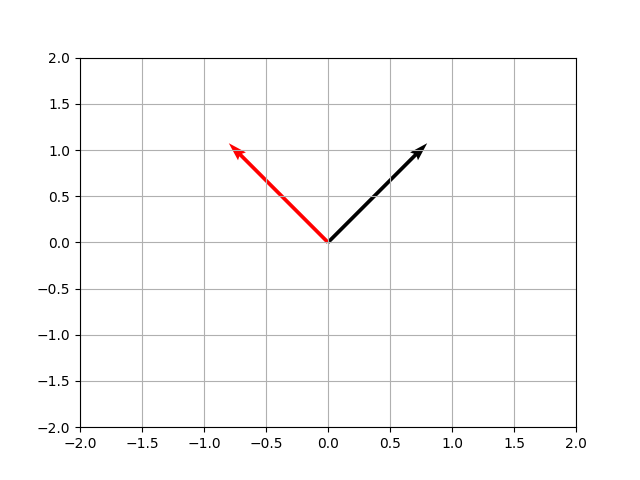
\includegraphics[width=20em]{phy_072_rot_04.png}

Doksan derece dönüş görülüyor.

Peki doksan derece değil $\theta$ kadar bir saat yönü tersi döndürüşü
nasıl temsil edilebilirdi? Yine bazın nereye gittiğine bakıyoruz,

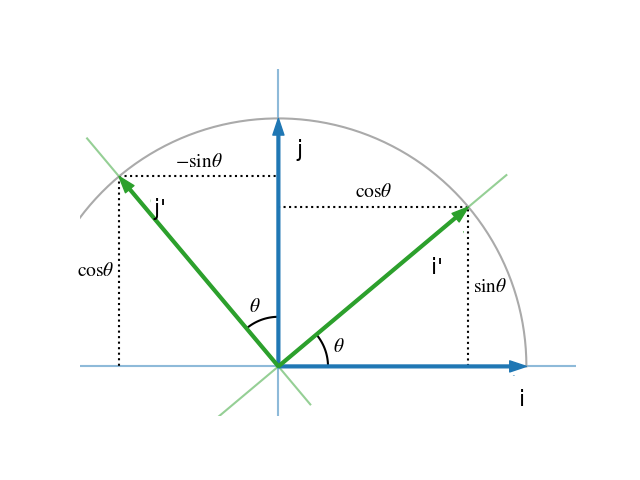
\includegraphics[width=20em]{phy_072_rot_03.png}

Eğer $i$'yi kaldırıp $i'$ haline getirirsek bu yeni vektörün
$[\cos\theta,\sin\theta]$ durumuna gelmesi, $j$'yi döndürüp $j'$ yapınca
$[-\sin\theta,\cos\theta]$ haline gelmesi demektir. Dönüş matrisi,

$$
R = \left[\begin{array}{rr}
\cos\theta & -\sin\theta \\
\sin\theta & \cos\theta
\end{array}\right]
$$

\begin{minted}[fontsize=\footnotesize]{python}
theta = np.deg2rad(20)
v = np.array([1,1])
plt.quiver(0,0,v[0],v[1],scale=5)
R = np.array([[np.cos(theta), -np.sin(theta)],[np.sin(theta),np.cos(theta)]])
vnew = np.dot(R, v)
plt.quiver(0,0,vnew[0],vnew[1],scale=5,color='red')
plt.xlim(-2,2)
plt.ylim(-2,2)
plt.grid(True)
plt.savefig('phy_072_rot_05.png')
\end{minted}

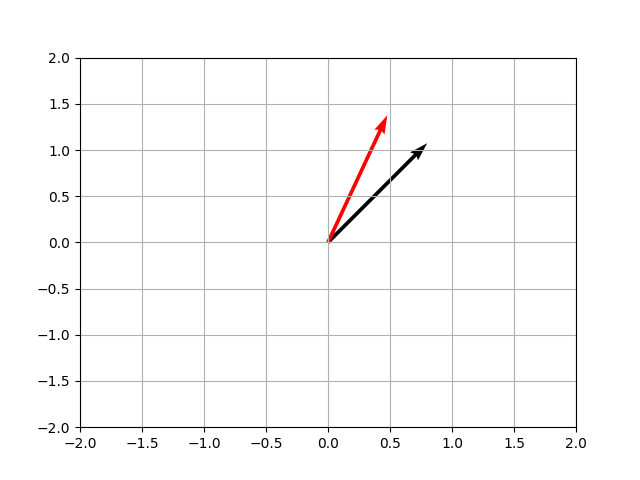
\includegraphics[width=20em]{phy_072_rot_05.png}

Euler Acıları (Euler Angles)

Bir katı gövdenin, ya da aeoridinamik simülasyonda uçağın, bir arabanın hangi
yöne baktığını (orientatıon) temsil etmek için Euler açıları yaygın şekilde
kullanılır. Bu açılar herhangi bir, ne kadar çetrefil olursa olsun dönüşün,
peşpeşe, her eksen etrafında uygulanabilecek üç tane ardı ardına yapılan
döndürme  ile temsil edilebileceğinden hareketle bulunmuştur. Mesela altta
ardı ardına YXZ eksenleri üzerinde yapılan döndürme gösteriliyor.

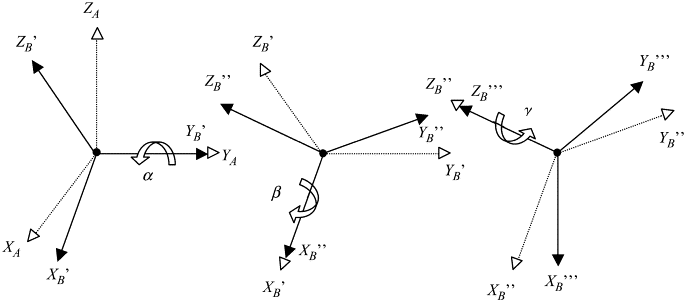
\includegraphics[width=20em]{phy_072_rot_06.png}

Genelde kullanım kalıbı ZYX ya da ZXZ üzerinden yapılır. Altta ZXZ ornegini
gorecegiz. Herhangi bir eksen etrafındaki dönüş tek bir dönüş matrisi ile
gösterilebilir, mesela Z etrafındaki $\phi$ kadar bir dönüş $D$ matrisinde olsun
[1, sf 153],

$$
D = \left[\begin{array}{rrr}
\cos \phi & \sin\phi & 0 \\
-\sin \phi & \cos\phi & 0 \\
0 & 0 & 1
\end{array}\right]
$$

O zaman $z$ ekseni etrafındaki bir dönüş

$$
\bar{x}' = D \bar{x}
$$

yani $\bar{x} = [x, y, z]$ döndürülerek $\bar{x}' = [x', y', z']$ elde edildi.

Şimdi $x'$ ekseni etrafında $\theta$ kadar döndürüyoruz, bunu $C$ ile yapalım,

$$
C = \left[\begin{array}{rrr}
1 & 0 & 0 \\
0 & \cos\theta & \sin\theta \\
0 & -\sin\theta & \cos\theta
\end{array}\right]
$$

$$
\bar{x}'' = C \bar{x}'
$$

Ve son olarak $\bar{x}'' = [x'',y'',z'']$ içindeki $z''$ etrafında $\psi$ kadar
döndürüyoruz, bunu $B$ ile yapalım,

$$
B = \left[\begin{array}{rrr}
\cos \psi & \sin\psi & 0 \\
-\sin \psi & \cos\psi & 0 \\
0 & 0 & 1
\end{array}\right]
$$

$$
\bar{x}_f = B \bar{x}''
$$

Tüm bu matris çarpımlarını tek bir satırda

$$
\bar{x}_f =  B C D \bar{x}
$$

ile yapabilirdik, ya da

$$
\bar{x}_f =  A \bar{x}
$$

olarak ki $A = BCD$ olmak üzere.. Bu $A$ matrisinin içeriği neye benzerdi? Cebirsel
olarak $BCD$ çarpımını gerçekleştirince,

$$
A = \left[\begin{array}{ccc}
\cos\psi\cos\phi-\cos\theta\sin\phi\sin\psi &
\cos\psi\sin\phi + \cos\theta\cos\phi\sin\psi &
\sin\psi\sin\theta \\
-\sin\psi\cos\phi-\cos\theta\sin\phi\cos\psi &
-\sin\psi\sin\phi + \cos\theta\cos\phi\cos\psi &
\cos\psi\sin\theta \\
\sin\theta \sin\phi &
-\sin\theta\cos\phi &
\cos\theta
\end{array}\right]
$$

Not: dikkat edelim, eksenlerde ardı ardına yapılan rotasyonların birleşimi
sırabağımsız değil, mesela alttaki iki döndürme, aynı temel döndürmeleri
yapıyor olsalar da farklı sıralarda yaptıkları için farklı sonuçları veriyorlar,

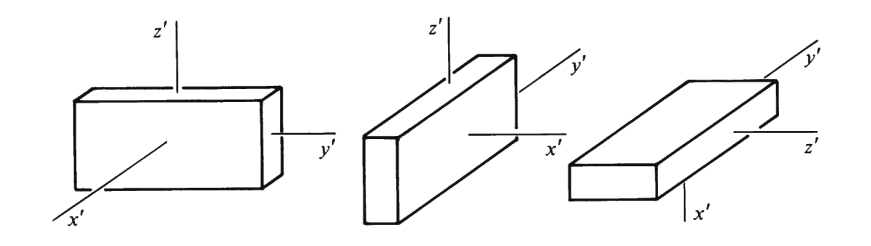
\includegraphics[width=20em]{phy_072_rot_01.png}

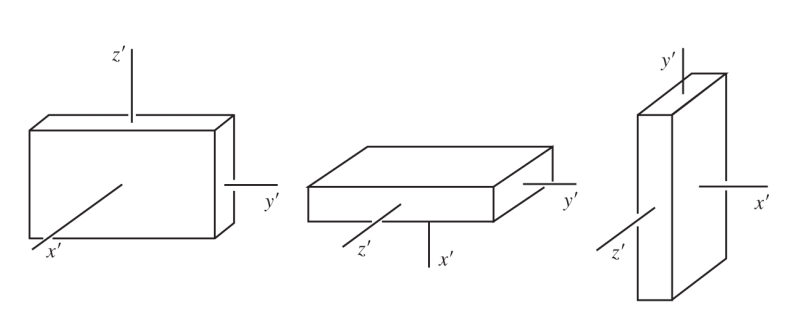
\includegraphics[width=20em]{phy_072_rot_02.png}

Tabii üstteki durum lineer cebirin içeriğiyle uyumlu, çünkü matris çarpımı da
sırabağımsız değildir.

Paket

Kütüphane \verb!scipy! içinde faydalı kodlar var, mesela \verb!scipy.spatial.transform!
içinde,

\begin{minted}[fontsize=\footnotesize]{python}
from scipy.spatial.transform import Rotation as R

r = R.from_euler('zyx', [90, 45, 30], degrees=True)
print (np.round(r.as_matrix(),2))
\end{minted}

\begin{verbatim}
[[ 0.   -0.71  0.71]
 [ 0.87 -0.35 -0.35]
 [ 0.5   0.61  0.61]]
\end{verbatim}

Diferansiyel Form, Sayisal Cozum






Kaynaklar

[1] Safko, {\em Classical Mechanics}

[2] Bayramlı, {\em Lineer Cebir, Giris}

[3] Widnall, {\em 16.07 Dynamics}

\end{document}




